\documentclass[cal1spr16Lectures.tex]{subfiles}

\begin{document}

%\section[Week 13]{Week 13: 18-22 Apr}

% % % 
\subsubsection{\bf Wednesday 20 April}
% % %

\begin{frame}[allowframebreaks]{Wed 20 Apr}
\begin{itemize}
\item Exam 3: Issue with increasing/decreasing, number lines, etc.  Point for signature.
\item April 22: Last day to drop with a "W".
\item Exam 4 next week, probably Friday.  Covers \S 4.7-5.4
\end{itemize}
\end{frame}

% % %
\begin{frame}\small
Without formally examining methods to evaluate definite integrals, we can use geometry.
\begin{exe} 
Using geometry, evaluate $\int_1^2 (4x-3)\ dx$. 

\vspace{0.5pc}
(\emph{Hint:}  The area of a trapezoid is $A=\frac{h(l_1+l_2)}{2}$, where $h$ is the height of the trapezoid and $l_1$ and $l_2$ are the lengths of the two parallel bases.)
\end{exe}
\end{frame}

% % %
\begin{frame}\footnotesize
\begin{exe} 
Using the picture below, evaluate the following definite integrals:
\[\text{1.\ } \int_0^a f(x)\ dx \qquad \text{2.\ } \int_0^b f(x)\ dx \qquad \text{3.\ } \int_0^c f(x)\ dx \qquad \text{4.\ } \int_a^c f(x)\ dx\]
\vspace{-2pc}

\begin{center}
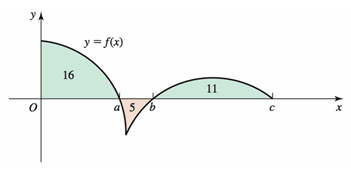
\includegraphics[scale=0.8]{pictures/Ch5Sect2_Exer31}
\end{center}
\end{exe}
\end{frame}

% % %
\subsubsection{Properties of Integrals}
% % %

% % %
\begin{frame}{\small Properties of Integrals}\footnotesize
\begin{itemize}
\item[1.] (Reversing Limits) $\int_b^a f(x)\ dx = -\int_a^b f(x)\ dx$

\vspace{0.75pc}
\item[2.] (Identical Limits) $\int_a^a f(x)\ dx = 0$

\vspace{0.75pc}
\item[3.] (Integral of a Sum) 

$\int_a^b (f(x)+g(x))\ dx = \int_a^b f(x)\ dx + \int_a^b g(x)\ dx$

\vspace{0.75pc}
\item[4.] (Constants in Integrals) $\int_a^b cf(x)\ dx = c \int_a^b f(x)\ dx$
\end{itemize}
\end{frame}

% % %
\begin{frame}{\small Properties of Integrals, cont.}\footnotesize
\begin{itemize}
\item[5.] (Integrals over Subintervals) If $c$ lies between $a$ and $b$, then
\[
\int_a^b f(x)\ dx = \int_a^c f(x)\ dx + \int_c^b f(x)\ dx.
\]

\item[6.] (Integrals of Absolute Values) The function $|f|$ is integrable on $[a,b]$ and $\int_a^b |f(x)|\ dx$ is the sum of the areas of regions bounded by the graph of $f$ and the $x$-axis on $[a,b]$.  (See Figure 5.31 on p.\ 329) 

\vspace{0.5pc}
\alert{(This is the total area, no negative signs.)}
\end{itemize}
\end{frame}

% % %
\begin{frame}\small
\begin{exe} 
If $\int_2^4 f(x)\ dx = 3$ and $\int_4^6 f(x)\ dx = -2$, then compute 
$\int_2^6 f(x)\ dx$. 
\end{exe}
\end{frame}

% % %
\subsubsection{Book Problems}
% % %

% % %
\begin{frame}
\begin{block}{5.2 Book Problems}
11-45 (odds), 67-74
\end{block}
\end{frame}

\subfile{5p3fundamentalTheoremOfCalculus}

\end{document}